\documentclass[a4paper,14pt]{article}
\usepackage{blindtext}
\usepackage[T2A]{fontenc}
\usepackage[utf8]{inputenc}
\usepackage[english,russian]{babel}
\usepackage{listings}
\usepackage{geometry}
\usepackage{amssymb}
\usepackage{amsmath}
\usepackage[14pt]{extsizes}
\geometry{left=3cm}
\geometry{right=1.5cm}
\geometry{top=2cm}
\geometry{bottom=2cm}
\pagestyle{plain}
\usepackage{pgfplots}
\usepackage{filecontents}
\usepackage{graphicx}
\usepackage{indentfirst}
\DeclareGraphicsExtensions{.png}
\graphicspath{{images/}}
\usetikzlibrary{datavisualization}
\usetikzlibrary{datavisualization.formats.functions}
\usepackage{tabularx}
\pgfplotsset{width=7 cm}
\usepackage{xcolor}
%\renewcommand{\rmdefault}{ftm}
%\usepackage{mathptmx}
\usepackage{setspace}
% \usepackage{minted}

%\полуторный интервал
\onehalfspacing
\frenchspacing

\usepackage{tocloft}
\frenchspacing
\setcounter{page}{2}
\usepackage{multirow}
\usepackage{float}
\usepackage{multirow}

\renewcommand{\cftsecdotsep}{\cftdot}
\renewcommand{\cftsecleader}{\cftdotfill{\cftsecdotsep}}
\renewcommand{\cftsubsecleader}{\cftdotfill{\cftsecdotsep}}
\renewcommand{\cftsubsubsecleader}{\cftdotfill{\cftsecdotsep}}

%\renewcommand\cftchapdotsep{\cftdot}
%\renewcommand\cftsecdotsep{\cftdot}
%\renewcommand{\cftchapleader}{\cftdotfill{\cftchapdotsep}}

% Для измененных титулов глав:
% % подключаем нужные пакеты
%\definecolor{gray75}{gray}{0.75} % определяем цвет
%\newcommand{\hsp}{\hspace{20pt}} % длина линии в 20pt
% titleformat определяет стиль
%\titleformat{\chapter}[hang]{\Huge\bfseries}{\thechapter\hsp\textcolor{black}{|}\hsp}{0pt}{\Huge\bfseries}
%\usepackage{titlesec, blindtext, color}
%\titleformat{\chapter}[hang]{\Huge\bfseries}{\thechapter\hsp\textcolor{black}{|}\hsp}{0pt}{\Huge\bfseries}

\lstset{ %
extendedchars=\true,
inputencoding=utf8,
morekeywords={include, printf},
texcl=\true,
breaklines=\true,
escapeend=\end{russian},
escapechar=\%,
keepspaces=\true,
language=python,                 % выбор языка для подсветки
basicstyle=\small\sffamily, % размер и начертание шрифта для подсветки кода
numbers=left,               % где поставить нумерацию строк (слева\справа)
numberstyle=\tiny,           % размер шрифта для номеров строк
stepnumber=1,                   % размер шага между двумя номерами строк
numbersep=5pt,                % как далеко отстоят номера строк от подсвечиваемого кода
showspaces=\true,            % показывать или нет пробелы специальными отступами
showstringspaces=\true,      % показывать или нет пробелы в строках
showtabs=false,             % показывать или нет табуляцию в строках
frame=single,              % рисовать рамку вокруг кода
tabsize=4,                 % размер табуляции по умолчанию равен 2 пробелам
captionpos=t,              % позиция заголовка вверху [t] или внизу [b]
breaklines=true,           % автоматически переносить строки (да\нет)
breakatwhitespace=false, % переносить строки только если есть пробел
escapeinside={\#*}{*)}   % если нужно добавить комментарии в коде
}



\begin{document}
\pgfplotsset{compat=1.17}

\begin{titlepage}

    \begin{table}
        \centering
        \footnotesize
        \begin{tabular}{cc}
            \multirow{8}{*}{
\includegraphics[scale=0.35]{bmstu.jpg}}
            & \\
            & \\
            & \textbf{Министерство науки и высшего образования Российской Федерации} \\
            & \textbf{Федеральное государственное бюджетное образовательное учреждение} \\
            & \textbf{высшего образования} \\
            & \textbf{<<Московский государственный технический} \\
            & \textbf{университет имени Н.Э. Баумана>>} \\
            & \textbf{(МГТУ им. Н.Э. Баумана)} \\
        \end{tabular}
    \end{table}

    \vspace{-2.5cm}

    \begin{flushleft}
        \rule[-1cm]{\textwidth}{3pt}
        \rule{\textwidth}{1pt}
    \end{flushleft}

    \begin{flushleft}
		ФАКУЛЬТЕТ Информатика и системы управления 
	\end{flushleft}
        КАФЕДРА Программное обеспечение ЭВМ и информационные технологии

    \vspace{3cm}

    \begin{center}
		\textbf{Лабораторная работа № 4} \\
		\textbf{Дисциплина: <<Моделирование>>}
        \vspace{0.5cm}
	\end{center}

	\begin{center}
		\textbf{Тема: <<Программно-алгоритмическая реализация моделей на основе дифференциальных уравнений в частных производных  с краевыми условиями II и  III рода>>}
        \vspace{0.5cm}
    \end{center}

    \vspace{2cm}

	\begin{flushleft}
        \begin{tabular}{ll}
            \textbf{Студент} & Овчинникова А. П. \\
            \textbf{Группа} & ИУ7-65Б \\
            \textbf{Оценка (баллы)} & \\
            \textbf{Преподаватель} & Градов В.М.   \\
        \end{tabular}
    \end{flushleft}

    \vspace{2cm}

   \begin{center}
        Москва, 2020 г.
    \end{center}

\end{titlepage}

\setcounter{page}{2}

\subsection*{Цель работы}

Целью данной работы является получение навыков 
разработки  алгоритмов решения смешанной краевой
 задачи при реализации моделей, построенных на 
 квазилинейном уравнении параболического типа. 

\subsection*{Исходные данные}

1. Задана математическая модель.

Уравнение для функции $T(x)$:

\begin{equation}
	c(T) \frac{\delta T}{\delta t} = \frac{\delta}{\delta x} \left( k(T) \frac{\delta T}{\delta x} \right) - \frac{2}{R} \alpha (x) T + \frac{2 T_0}{R} \alpha(x)
\end{equation}

Краевые условия

\begin{equation}
	\begin{cases}
		t = 0, T(x, 0) = T_0 \\
		x = 0, -k(T(0)) \frac{\delta T}{\delta x} = F_0 \\
		x = l, -k(T(l)) \frac{\delta T}{\delta x} = \alpha_N (T(l) - T_0)
  	\end{cases}
\end{equation}

Примем

\begin{eqnarray}
	p(x) = \frac{2}{R} \alpha(x) \\
	f(u) = f(x) = \frac{2 T_0}{R} \alpha(x) \\
	F = -k(T) \frac{\delta T}{\delta x}
\end{eqnarray}

2. Разностная схема:

\begin{eqnarray}
	\stackrel{\frown}{A}_n \stackrel{\frown}{y}_{n-1} - \stackrel{\frown}{B}_n \stackrel{\frown}{y}_n + \stackrel{\frown}{D}_n \stackrel{\frown}{y}_{n+1} = - \stackrel{\frown}{F}_n, 1 \leq n \leq N - 1
\end{eqnarray}

где

\begin{equation}
	\stackrel{\frown}{A}_n = \stackrel{\frown}{\chi}_{n-1/2} \frac{\tau}{h}, 
\end{equation}

\begin{equation}
	\stackrel{\frown}{D}_n = \stackrel{\frown}{\chi}_{n+1/2} \frac{\tau}{h},
\end{equation}

\begin{equation}
	\stackrel{\frown}{B}_n = \stackrel{\frown}{A}_n + \stackrel{\frown}{D}_n + \stackrel{\frown}{c}_n h + \stackrel{\frown}{p}_n h \tau,
\end{equation}

\begin{equation}
	\stackrel{\frown}{F}_n = f_n h \tau + \stackrel{\frown}{c}_n y_n h.
\end{equation}

Разностный аналог краевого условия при $x = 0$ (получена в Лекции №14 (14.6),(14.7)):

\begin{eqnarray}
	\left( \frac{h}{8} \stackrel{\frown}{c}_{1/2} + \frac{h}{4} \stackrel{\frown}{c}_0 + \stackrel{\frown}{\chi}_{1/2} \frac{\tau}{h} + \frac{\tau h}{8} p_{1/2} + \frac{\tau h}{4} p_0 \right) \stackrel{\frown}{y}_0 + \nonumber \\ 
	+ \left( \frac{h}{8} \stackrel{\frown}{c}_{1/2} - \stackrel{\frown}{\chi}_{1/2} \frac{\tau}{h} + \frac{\tau h}{8} p_{1/2} \right) \stackrel{\frown}{y}_1 = \nonumber \\
	= \frac{h}{8} \stackrel{\frown}{c}_{1/2} (y_0 + y_1) + \frac{h}{4} \stackrel{\frown}{c}_0 y_0 + \stackrel{\frown}{F} \tau + \frac{\tau h}{4} (\stackrel{\frown}{f}_{1/2} + \stackrel{\frown}{f}_0)
\end{eqnarray}

Самостоятельно надо получить интегро-интерполяционным методом разностный аналог краевого условия при $x = l$.
При этом учесть, что поток

\begin{eqnarray}
	\stackrel{\frown}{F}_n = \alpha_N (\stackrel{\frown}{y}_N - T_0), \\
	\stackrel{\frown}{F}_{N - 1/2} = \stackrel{\frown}{\chi}_{N-1/2} \frac{\stackrel{\frown}{y}_{N-1} - \stackrel{\frown}{y}_N }{h}.
\end{eqnarray}

3. Значения параметров для отладки (все размерности согласованы).

\begin{table}[!h]
	\caption{\label{tab.canonsummary} Значения параматров.}
	\begin{center}
	\begin{tabular}{|c c|}
	\hline
	$k(T) = $ & $a_1 (b_1 + c_1 T^{m_1})$ Вт/см К \\
	$c(T) = $ & $a_2 + b_2 T^{m_2} - \frac{c_2}{T^2} $ Дж/см$^3$ К \\
	$a_1 = $ & 0.0134 \\
	$b_1 = $ & 1 \\
	$c_1 = $ & $4.35 \cdot 10^{-4} $ \\
	$m_1 = $ & 1 \\
	$a_2 = $ & 2.049 \\
	$b_2 = $ & $0.563 \cdot 10^{-3}$ \\
	$c_2 = $ & $0.528 \cdot 10^{5}$ \\
	$m_2 =$ & 1 \\
	$\alpha (x) =$ & $\frac{c}{x-d}$ \\
	$\alpha_0 =$ & 0.05 Вт/см$^2$ К \\
	$\alpha_N =$ & 0.01 Вт/см$^2$ К \\
	$l =$ & 10 см \\
	$T_0 =$ & 300 К \\
	$R =$ & 0.5 см \\
	$F(t) =$ & 50 Вт/см$^2$ \\
	\hline
	\end{tabular}
	\end{center}
	\end{table} 
	

\newpage
\subsection*{Физическое содержание задачи}

Постановки задач в данной лабораторной  работе и работе №3 во многом совпадают. Отличия заключаются в следующем.

\begin{enumerate}
	\item Сформулированная в данной работе  математическая модель описывает нестационарное температурное поле $T(x, t)$, зависящее от координаты x и меняющееся во времени.
	\item Свойства материала стержня привязаны к температуре, т.е. теплоемкость и коэффициент теплопроводности $c(T), k(T)$ зависят от $T$ , тогда как в работе №3 $k(x)$ зависит от координаты, а $c = 0$.
	\item При $x = 0$ цилиндр нагружается тепловым потоком $F(t)$ , в общем случае зависящим от времени, а в работе №3 поток был постоянный.
\end{enumerate}

Если в настоящей работе задать  поток постоянным, т.е. $F(t) = const$, то  будет происходить формирование температурного поля от начальной температуры
$T_0$ до некоторого установившегося (стационарного) распределения $T(x, t)$.
Это поле в дальнейшем с течением времени меняться не будет и  должно совпасть с температурным распределением $T(x)$, получаемым в лаб. работе №3, если все параметры задач совпадают, в частности, вместо
$k(T)$ надо использовать $k(x)$ из лаб. работы №3. Это полезный факт для тестирования программы.

Если после разогрева стержня положить поток $F(t) = 0$, то будет происходить остывание, пока температура не выровняется по всей длине и не станет равной $T_0$.

При произвольной зависимости потока $F(t)$ от времени температурное поле будет как-то сложным образом отслеживать поток.

\textbf{Замечание.} Варьируя параметры задачи, следует обращать внимание на то, что решения, в которых температура превышает примерно  2000К, физического смысла не имеют и практического интереса не представляют.

\subsection*{Задание}

\begin{enumerate}
	\item Представить разностный аналог краевого условия при  и его краткий вывод интегро -интерполяционным методом.
	\item График зависимости температуры $T(x, t_m)$ от координаты $x$ при нескольких фиксированных значениях времени $t_m$ 
	(аналогично рисунку в лекции №14)  при заданных выше параметрах. Обязательно представить распределение $T(x, t)$ в момент времени, соответствующий установившемуся режиму, когда поле перестает меняться с
	некоторой точностью, т.е. имеет место выход на стационарный режим. На этой стадии левая часть дифференциального уравнения близка к нулю, и на самом деле решается уравнение из лабораторной работы №3 (отличие только в том, что там было линейное уравнение).
	\item График зависимости $T(x_n, t)$ при нескольких фиксированных значениях координаты $x_n$. Обязательно представить случай $n = 0$, т.е. $x = x_0 = 0$.
\end{enumerate}


\subsection*{Предварительные вычисления}

\textbf{1. Найдем $c, d$.}

$c = -\alpha_0 d$

$d = \frac{\alpha_N l}{\alpha_N - \alpha_0}$.

\textbf{2. Получим интегро-интерполяционным методом разностный
аналог краевого условия при $x = l$.}

Запишем уравнение (1) с учетом (3), (4) и (5)

\begin{equation}
	c(T) \frac{\delta T}{\delta x} = - \frac{\delta F}{\delta x} - p(x) T + f(T)
\end{equation}


Проводим интегрирование уравнения (14) на отрезке $[x_{N-1/2}; x_N]$
и на временном интервале $[t_m; t_{m+1}]$.

 \begin{eqnarray}
	\int\limits_{x_{N-1/2}}^{x_N} dx \int\limits_{t_m}^{t_{m+1}} c(T) \frac{\delta T}{\delta t} dt = \nonumber \\
	= - \int\limits_{t_m}^{t_{m+1}} dt \int\limits_{x_{N-1/2}}^{x_N} \frac{\delta F}{\delta x} dx - \int\limits_{x_{N-1/2}}^{x_N} dx \int\limits_{t_m}^{t_{m+1}} p(x) T dt + \int\limits_{x_{N-1/2}}^{x_N} dx \int\limits_{t_m}^{t_{m+1}} f(T) dt
 \end{eqnarray}

или

\begin{eqnarray}
	\int\limits_{x_{N-1/2}}^{x_N} \stackrel{\frown}{c} (\stackrel{\frown}{T} - T) dx = \int\limits_{t_m}^{t_{m+1}} (F_{N} - F_{N-1/2}) dt - \int\limits_{x_{N-1/2}}^{x_N} p \stackrel{\frown}{T} \tau dx + \nonumber \\
	+ \int\limits_{x_{N-1/2}}^{x_N} \stackrel{\frown}{f} \tau dx
\end{eqnarray}

Здесь  при  вычислении  внутренних  интегралов  по $t$ справа  в  уравнении (15)
применен метод правых прямоугольников, тем самым следует ожидать порядок точности 
$O(\tau)$ по переменной $t$.

Вычисляем интегралы. Первый интеграл  справа,как и ранее, находим методом правых прямоугольников, а остальные -- методом трапеций.

\begin{eqnarray}
	\frac{h}{4} \left( \stackrel{\frown}{c}_N (\stackrel{\frown}{y}_N - y_N) + \stackrel{\frown}{c}_{N-1/2} (\stackrel{\frown}{y}_{N-1/2} - y_{N-1/2}) \right) = - (\stackrel{\frown}{F}_N - \stackrel{\frown}{F}_{N-1/2}) \tau - \nonumber \\
	- (p_N \stackrel{\frown}{y}_N + p_{N-1/2} \stackrel{\frown}{y}_{N-1/2} ) \tau \frac{h}{4} + (\stackrel{\frown}{f}_N + \stackrel{\frown}{f}_{N-1/2}) \tau \frac{h}{4}.
\end{eqnarray}

Подставляя  в  данное  уравнение (12) и (13), и заменяя
$\stackrel{\frown}{y}_{N-1/2} = \frac{ \stackrel{\frown}{y}_{N-1} + \stackrel{\frown}{y}_N }{2}$, 
$y_{N-1/2} = \frac{y_{N-1} + y_N}{2}$, найдем разностный аналог краевого условия.

\begin{eqnarray}
	\stackrel{\frown}{y}_{N-1} \left( \frac{h}{8} \stackrel{\frown}{c}_{N-1/2} - \frac{\tau \stackrel{\frown}{\chi}_{N-1/2} }{h} + \frac{h}{8} p_{N-1/2} \right) + \nonumber \\
	+ \stackrel{\frown}{y}_N \left( \frac{h}{4} \stackrel{\frown}{c}_N + \frac{h}{8} \stackrel{\frown}{c}_{N-1/2} + \tau \alpha_N + \frac{\tau \stackrel{\frown}{\chi}_{N-1/2}}{h} + \frac{h}{4} \tau p_N + \frac{h}{8} \tau p_{N-1/2} \right) = \nonumber \\
	= \frac{h}{4} \stackrel{\frown}{c}_N y_N + \frac{h}{8} \stackrel{\frown}{c}_{N-1/2} y_N + \nonumber \\
	+ \frac{h}{8} \stackrel{\frown}{c}_{N-1/2} y_{N-1} + \tau \alpha_N T_0 + \frac{h}{4} \tau \left( \stackrel{\frown}{f}_N + \stackrel{\frown}{f}_{N-1/2} \right)
\end{eqnarray}

Отсюда ищутся начальные значения прогоночных коэффициентов.

В итоге система квазилинейных разностных уравнений примет канонический вид

\begin{equation}
	\begin{cases}
		\stackrel{\frown}{K}_0 \stackrel{\frown}{y}_0 + \stackrel{\frown}{M}_0 \stackrel{\frown}{y}_1 = \stackrel{\frown}{P}_0, \\
		\stackrel{\frown}{A}_n \stackrel{\frown}{y}_{n-1} - \stackrel{\frown}{B}_n \stackrel{\frown}{y}_n + \stackrel{\frown}{D}_n \stackrel{\frown}{y}_{n+1} = - \stackrel{\frown}{F}_n, 1 \leq n \leq N-1, \\
		\stackrel{\frown}{K}_N \stackrel{\frown}{y}_N + \stackrel{\frown}{M}_{N-1} \stackrel{\frown}{y}_{N-1} = \stackrel{\frown}{P}_N.
	\end{cases}
\end{equation}

Система (19) решается методом простых итераций. В методе простых итераций система (19)
решается многократно на каждом шаге по времени, т.е. для получения решения 
$\stackrel{\frown}{y}_n, n = 0...N$ в момент времени $t = t_{m+1}$ итера-ционная процедура организуется по схеме (8.3) из лекции №8.

\begin{eqnarray}
	\stackrel{\frown}{A}_n^{s-1} \stackrel{\frown}{y}_{n+1}^s - \stackrel{\frown}{B}_n^{s-1} \stackrel{\frown}{y}_n^s + \stackrel{\frown}{D}_n^{s-1} \stackrel{\frown}{y}_{n-1}^s = - \stackrel{\frown}{F}_n^{s-1},
\end{eqnarray}

здесь $s$ -- номер итерации.

В  качестве  начального  приближения $\stackrel{\frown}{y}_n^0$ задается  сошедшееся  решение 
$\stackrel{\frown}{y}_n$ с предыдущего шага $t = t_m$, то есть $\stackrel{\frown}{y}_n^0 = \stackrel{\frown}{y}_n$.

Прекращение итераций происходит при условиями

\begin{equation}
	max \left| \frac{\stackrel{\frown}{y}_n^s - \stackrel{\frown}{y}_n^{s-1}}{\stackrel{\frown}{y}_n^s} \right| \leq \varepsilon.
\end{equation}

В  итоге  для  каждого  момента  времени $t = t_m, m = 1, 2, ... M$ получаем  разностное решение
$\stackrel{\frown}{y}_n$. Набор таких решений для всех $t = t_m, m = 1, 2, ... M$ оответствуетфункции двух переменных 
$T(x_n, t_m)$, являющейся решением исходного  дифференциального  уравнения (1).

\subsection*{Код программы}

Код программы представлен в листингах 1-2.

\begin{lstlisting}[label=code1,caption=\text{Класс MyApp.}]
	import sys

	from PyQt5 import QtWidgets
	from PyQt5.QtWidgets import QMessageBox
	
	from Ui_mainwindow import Ui_MainWindow
	
	from Modeller import Modeller
	
	class MyApp(QtWidgets.QMainWindow):
		def __init__(self):
			super(MyApp, self).__init__()
			self.ui = Ui_MainWindow()
			self.ui.setupUi(self)
	
			self.ui.set_def_button.clicked.connect(self.set_defaults)
			self.ui.run_button.clicked.connect(self.run)
	
			self.defaults = {
				"a1" 	 : 0.0134,
				"b1" 	 : 1,
				"c1" 	 : 4.35e-4,
				"m1" 	 : 1,
				"a2" 	 : 2.049,
				"b2" 	 : 0.563e-3,
				"c2" 	 : 0.528e5,
				"m2" 	 : 1,
				"alpha0" : 0.05,
				"alphaN" : 0.01,
				"l"	 	 : 10,
				"T0"	 : 300,
				"R"		 : 0.5,
				"F0"	 : 50,
				"h"		 : 0.001,
				"t"		 : 1
			}
	
			self.data = {
				"a1" 	 : None,
				"b1" 	 : None,
				"c1" 	 : None,
				"m1" 	 : None,
				"a2" 	 : None,
				"b2" 	 : None,
				"c2" 	 : None,
				"m2" 	 : None,
				"alpha0" : None,
				"alphaN" : None,
				"l"	 	 : None,
				"T0"	 : None,
				"R"		 : None,
				"F0"	 : None,
				"h"		 : None,
				"t"		 : None
			}
	
			self.set_defaults()
		
		def set_defaults(self):
			self.ui.lineEdit_a1.setText(str(self.defaults.get("a1")))
			self.ui.lineEdit_b1.setText(str(self.defaults.get("b1")))
			self.ui.lineEdit_c1.setText(str(self.defaults.get("c1")))
			self.ui.lineEdit_m1.setText(str(self.defaults.get("m1")))
	
			self.ui.lineEdit_a2.setText(str(self.defaults.get("a2")))
			self.ui.lineEdit_b2.setText(str(self.defaults.get("b2")))
			self.ui.lineEdit_c2.setText(str(self.defaults.get("c2")))
			self.ui.lineEdit_m2.setText(str(self.defaults.get("m2")))
	
			self.ui.lineEdit_alpha0.setText(str(self.defaults.get("alpha0")))
			self.ui.lineEdit_alphaN.setText(str(self.defaults.get("alphaN")))
	
			self.ui.lineEdit_l.setText(str(self.defaults.get("l")))
			self.ui.lineEdit_T0.setText(str(self.defaults.get("T0")))
			self.ui.lineEdit_R.setText(str(self.defaults.get("R")))
			self.ui.lineEdit_F0.setText(str(self.defaults.get("F0")))
	
			self.ui.lineEdit_h.setText(str(self.defaults.get("h")))
			self.ui.lineEdit_t.setText(str(self.defaults.get("t")))
	
		def get_data(self):
			try:
				self.data["a1"] = float(self.ui.lineEdit_a1.text())
				self.data["b1"] = float(self.ui.lineEdit_b1.text())
				self.data["c1"] = float(self.ui.lineEdit_c1.text())
				self.data["m1"] = float(self.ui.lineEdit_m1.text())
	
				self.data["a2"] = float(self.ui.lineEdit_a2.text())
				self.data["b2"] = float(self.ui.lineEdit_b2.text())
				self.data["c2"] = float(self.ui.lineEdit_c2.text())
				self.data["m2"] = float(self.ui.lineEdit_m2.text())
	
				self.data["alpha0"] = float(self.ui.lineEdit_alpha0.text())
				self.data["alphaN"] = float(self.ui.lineEdit_alphaN.text())
	
				self.data["l"] = float(self.ui.lineEdit_l.text())
				self.data["T0"] = float(self.ui.lineEdit_T0.text())
				self.data["R"] = float(self.ui.lineEdit_R.text())
				self.data["F0"] = float(self.ui.lineEdit_F0.text())
	
				self.data["h"] = float(self.ui.lineEdit_h.text())
				self.data["t"] = float(self.ui.lineEdit_t.text())
	
			except ValueError:
				return False
			return True
	
		def run(self):
			if self.get_data():
				print("Computing...")
				mdlr = Modeller(self.data)
				mdlr.compute()
				print("Finish.")
			else:
				self.msg_box("Error!", "Error! Incorrect input!", QMessageBox.Critical)
	
		def msg_box(self, title, message, type):
			msg = QMessageBox(self)
			msg.setIcon(type)
			msg.setWindowTitle(title)
			msg.setText(message)
			msg.addButton('Ok', QMessageBox.AcceptRole)
			msg.exec()
	
	
	def main():
		app = QtWidgets.QApplication(sys.argv)
		window = MyApp()
		window.show()
		app.exec_()
	
	
	if __name__ == '__main__':
		main()	
\end{lstlisting}

\begin{lstlisting}[label=code1,caption=\text{Класс Modeller.}]
	import matplotlib.pyplot as plt
	import numpy as np
	from math import fabs
	
	class Modeller():
		def __init__(self, data):
			self.data = data
	
			self.a1 = self.data.get("a1")
			self.b1 = self.data.get("b1")
			self.c1 = self.data.get("c1")
			self.m1 = self.data.get("m1")
	
			self.a2 = self.data.get("a2")
			self.b2 = self.data.get("b2")
			self.c2 = self.data.get("c2")
			self.m2 = self.data.get("m2")
			
			self.alpha0 = self.data.get("alpha0")
			self.alphaN = self.data.get("alphaN")
	
			self.l = self.data.get("l")
			self.T0 = self.data.get("T0")
			self.R = self.data.get("R")
			self.F0 = self.data.get("F0")
	
			self.h = self.data.get("h")
			self.t = self.data.get("t")
	
			self.d = (self.alphaN * self.l) / (self.alphaN - self.alpha0)
			self.c_koef = - self.alpha0 * self.d
	
			self.eps = 1e-2
	
		def c(self, T):
			res = self.a2 + self.b2 * (T ** self.m2) - (self.c2 / (T ** 2))
			return res
			#return 0
	
		def f_plus_half(self, x, h, func):
			res = (func(x) + func(x + h)) / 2
			return res
		
		def f_minus_half(self, x, h, func):
			res = (func(x) + func(x - h)) / 2
			return res
		
		def old_k(self, x):
			res = self.a1 / (x - self.b1)
			return res
	
		def k(self, T):
			#res = self.old_k(self.x)
			res = self.a1 * (self.b1 + self.c1 * (T ** self.m1))
			return res
	
		def alpha(self, x):
			return self.c_koef / (x - self.d)
	
		def p(self, x):
			return 2 * self.alpha(x) / self.R
	
		def f(self, x):
			return 2 * self.alpha(x) * self.T0 / self.R
	
		def __left_boundary_condition(self, T):
			h8 = self.h / 8
			h4 = self.h / 4
			h2 = self.h / 2
			c_p12 = self.f_plus_half(T[0], self.t, self.c)
			chi_p12 = self.f_plus_half(T[0], self.t, self.k)
			t_over_h = self.t / self.h
	
			K0 = h8 * c_p12 + \
				 h4 * self.c(T[0]) + chi_p12 * t_over_h + \
				 self.t * h8 * self.p(h2) + (self.t * self.h) / 4 * self.p(0)
	
			M0 = h8 * c_p12 - chi_p12 * t_over_h + \
				 self.t * h8 * self.p(h2)
	
			P0 = h8 * c_p12 * (T[0] + T[1]) + \
				 h4 * self.c(T[0]) * T[0] + self.F0 * self.t + \
				 self.t * h8 * (3 * self.f(0) + self.f(self.h))
				 #self.t * h4 * (self.f(0) + self.f_plus_half(T[0], self.t, self.f)) # ?
			return K0, M0, P0
	
		def __right_boundary_condition(self, T):
			h8 = self.h / 8
			h4 = self.h / 4
			h2 = self.h / 2
			c_m12 = self.f_minus_half(T[-1], self.t, self.c)
			chi_m12 = self.f_minus_half(T[-1], self.t, self.k)
	
			h8_cm12 = h8 * c_m12 
	
			KN = h4 * self.c(T[-1]) + h8_cm12 + \
				self.t * self.alphaN + self.t * chi_m12 / self.h + \
				h4 * self.t * self.p(self.l) + h8 * self.t * self.p(self.l - h2)
			
			MN = h8_cm12 - \
				  self.t * chi_m12 / self.h + \
				  h8 * self.p(self.l - h2)
				
			PN = h4 * self.c(T[-1]) * T[-1] + h8_cm12 * T[-1] +\
				  h8_cm12 * T[-2] + \
				  self.t * self.alphaN * self.T0 + \
				  h4 * self.t * (self.f(self.l) + self.f(self.l - h2))
			
			return KN, MN, PN
	
		def A(self, T):
			return self.t / self.h * self.f_minus_half(T, self.t, self.k)
	
	
		def D(self, T):
			return self.t / self.h * self.f_plus_half(T, self.t, self.k)
	
		def B(self, x, T):
			return self.A(T) + self.D(T) + self.c(T) * self.h + \
				 self.p(x) * self.h * self.t
	
		def F(self, x, T):
			return self.f(x) * self.h * self.t + self.c(T) * T * self.h
	
		def progon(self, T, K0, M0, P0, KN, MN, PN):
			epsilon = [0, - M0 / K0]
			eta = [0, P0 / K0]
	
			x = self.h
			n = 1
			while x + self.h < self.l:
				An = self.A(T[n])
				Bn = self.B(x, T[n])
	
				newEps = self.D(T[n]) / (Bn - An * epsilon[n])
				epsilon.append(newEps)
	
				newEta = (self.F(x, T[n]) + An * eta[n]) / (Bn - An * epsilon[n])
				eta.append(newEta)
	
				x += self.h
				n += 1
			
			T = [0] * (n + 1)
			T[n] = (PN - MN * eta[n]) / (KN + MN * epsilon[n])
	
			for i in range(n-1, -1, -1):
				T[i] = epsilon[i + 1] * T[i + 1] + eta[i+1]
	
			return T
	
		def check_iter(self, T, T_next):
			#если нагрев 	замедлилися	и	изменение	температуры	за 
			#шаг по	времени	достаточно	мало
			max = fabs((T[0] - T_next[0]) / T_next[0])
			for i, j in zip(T, T_next):
				d = fabs(i - j) / j
				if d > max:
					max = d
			return max < 1
	
		def check_epsilon(self, T, T_next):
			#если	максимально	изменившийся	элемент
			#изменился меньше, чем	на eps
			for i, j in zip(T, T_next):
				
				if fabs((i - j) / j) > self.eps:
					return True
			return False
	
		def __iterate(self):
			res = []
			n = int(self.l / self.h)
			print(n)
			T = [self.T0] * (n + 1)
			T_new = [0] * (n + 1)
			ti = 0
			res.append(T)
			while True:
				tmp = T
				self.x = self.h
				while True:
					K0, M0, P0 = self.__left_boundary_condition(tmp)
					KN, MN, PN = self.__right_boundary_condition(tmp)
					T_new = self.progon(tmp, K0, M0, P0, KN, MN, PN)
					self.x += self.h
	
					if self.check_iter(tmp, T_new):
						break
					tmp = T_new
	
				res.append(T_new)
				ti += self.t
				if not self.check_epsilon(T, T_new):
					break
				T = T_new
			return res, ti
	
		def compute(self):
			res, ti = self.__iterate()
	
			xes = [i for i in np.arange(0, self.l, self.h)]
			#ts = [i for i in range(0, int(ti), int(self.t))]
			ts = [i for i in np.arange(0, ti, self.t)]
			
			s = 0
			for i in res:	
				if s % 2 == 0:
					plt.plot(xes, i[:-1])
				s += 2
	
			plt.plot(xes, res[-1][:-1], 'r')
			plt.xlabel("x, см")
			plt.ylabel("T, К")
			plt.grid()
			plt.show()
	
			s = 0
			while s < self.l / 3:
				p = [j[int(s / self.h)] for j in res]
				plt.plot(ts, p[:-1])
				s += 0.1
			plt.xlabel("t, sec")
			plt.ylabel("T, K")
			plt.grid()
			plt.show()	
\end{lstlisting}

\newpage
\subsection*{Результаты работы программы}

1. Представить разностный аналог краевого условия при  и его краткий вывод интегро-интерполяционным методом.

Вывод был проведен выше в разделе <<Предварительные вычисления>>.

2. График зависимости $T(x_n, t)$ при нескольких
фиксированных значениях координаты $x_n$.

\begin{figure}[!h]
	\center{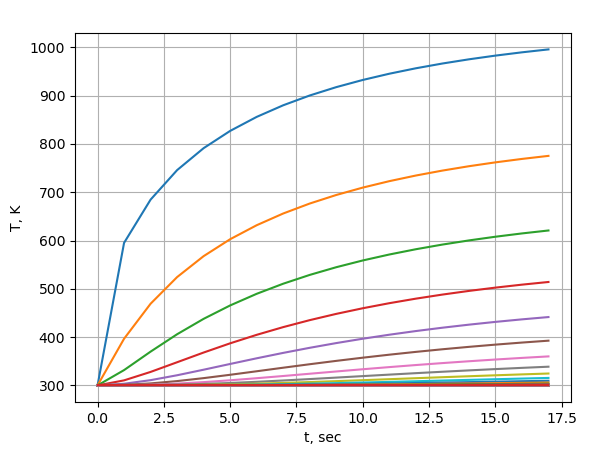
\includegraphics[width=15cm]{r2}}
	\caption{График зависимости $T(x_n, t)$ при нескольких
	фиксированных значениях координаты $x_n$.}
	\label{fig:image}
\end{figure}

3. График зависимости температуры $T(x, t_m)$ от координаты
$x$ при нескольких фиксированных значениях времени $t_m$.

На рисунке 2 красным цветом представлено распределение
$T(x, t_m)$ в момент времени, соответсвтующий
установившемуся режиму, когда поле перестает меняться с
некоторой точностью (1e-2), т.е. имеет место выход на стационарный режим.


\begin{figure}[!h]
	\center{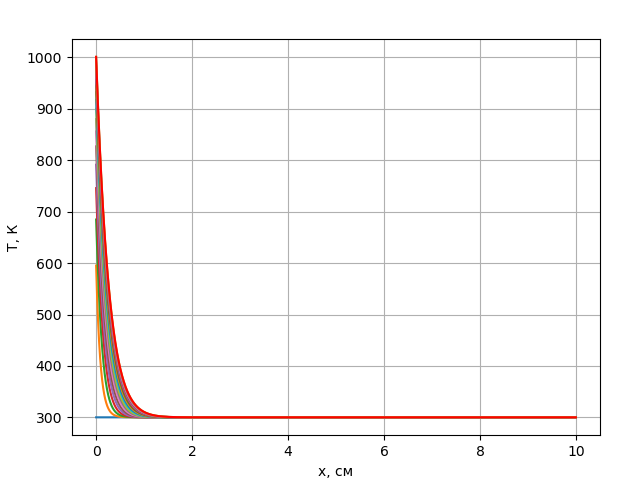
\includegraphics[width=15cm]{r1}}
	\caption{График зависимости температуры $T(x, t_m)$ от координаты
	$x$ при нескольких фиксированных значениях времени $t_m$.}
	\label{fig:image}
\end{figure}

\newpage
\subsection*{Ответы на вопросы}

\textbf{1. Приведите результаты тестирования программы (графики, общие соображения, качественный анализ). Учесть опыт выполнения лабораторной работы №3.}

1. Если после разогрева стержня положить поток $F(t) = 0$, то будет происходить остывание, пока 
температура не выровняется по всей длине и не станет равной $T_0$ (рисунок 3).

\begin{figure}[!h]
	\center{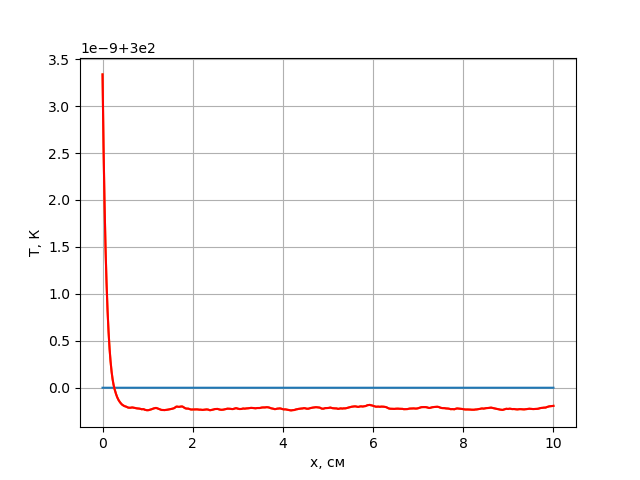
\includegraphics[width=15cm]{r3}}
	\caption{$F(t) = 0$.}
	\label{fig:image}
\end{figure}

\newpage
2. Если в настоящей работе задать поток постоянным, т.е. $F(t) = const$,
то будет происходить формирование температурного поля от начальнойтемпературы $T0$ 
до некоторого установившегося (стационарного) распределения $T(x,t)$. 
Это поле в дальнейшем с течением времени меняться не 
будет и должно совпасть с температурным распределением $T(x)$, 
получаемым в лаб. работе №3, если все параметры задач совпадают, 
в частности, вместо $k(T)$ надо использовать $k(x)$ из лаб. работы №3.

Необходимо задать $a_1 = 1.333$ и $b_1 = -3.333$, как в лабораторной №3.

На рисунке 4 представлен полученный график. 

График из 3 лабораторной для сравнения приведен на рисунке 5.

\newpage
\begin{figure}[!h]
	\center{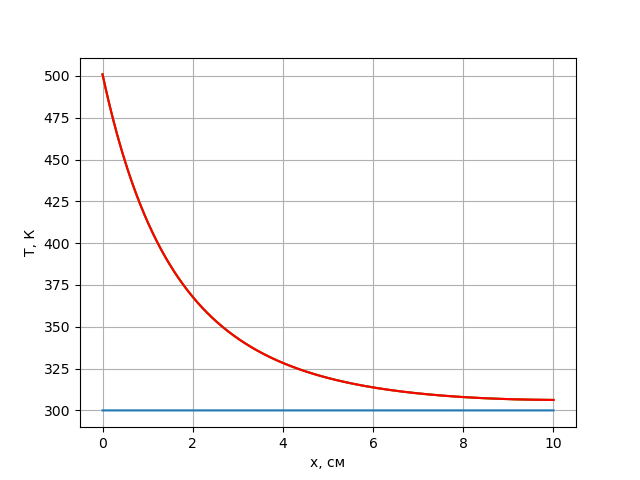
\includegraphics[width=15cm]{Fr4}}
	\caption{$k(x)$ вместо $k(T)$.}
	\label{fig:image}
\end{figure}

\newpage
\begin{figure}[!h]
	\center{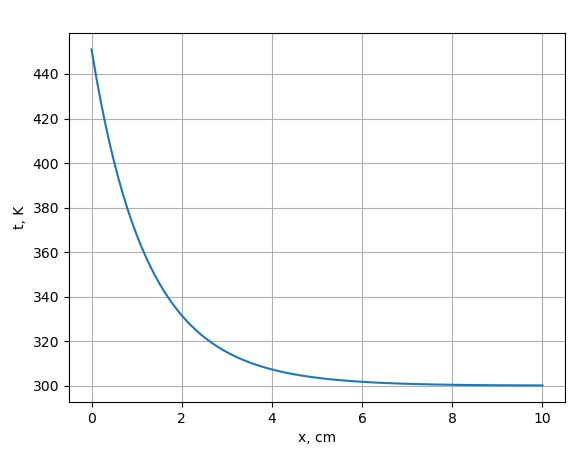
\includegraphics[width=15cm]{gr1}}
	\caption{График из лабораторной №3.}
	\label{fig:image}
\end{figure}

\newpage
\textbf{2. Выполните линеаризацию уравнения (14.8) по Ньютону, 
полагая для простоты, что все коэффициенты зависят только от одной 
переменной $\stackrel{\frown}{y}_n$. Приведите линеаризованный вариант уравнения и опишите алгоритм его решения. Воспользуйтесь процедурой вывода, описанной в лекции №8.}

Имеем:

\begin{equation}
	\begin{cases}
		\stackrel{\frown}{K}_0 \stackrel{\frown}{y}_0 + \stackrel{\frown}{M}_0 \stackrel{\frown}{y}_1 = \stackrel{\frown}{P}_0, \\
		\stackrel{\frown}{A}_n \stackrel{\frown}{y}_{n-1} - \stackrel{\frown}{B}_n \stackrel{\frown}{y}_n + \stackrel{\frown}{D}_n \stackrel{\frown}{y}_{n+1} = - \stackrel{\frown}{F}_n, 1 \leq n \leq N-1, \\
		\stackrel{\frown}{K}_N \stackrel{\frown}{y}_N + \stackrel{\frown}{M}_{N-1} \stackrel{\frown}{y}_{N-1} = \stackrel{\frown}{P}_N.
	\end{cases}
\end{equation}

Выполняя линеаризацию по Ньютону последовательно по неизвестным 

\begin{eqnarray}
	\left( \stackrel{\frown}{A}_n \stackrel{\frown}{y}_{n-1} - \stackrel{\frown}{B}_n \stackrel{\frown}{y}_n + \stackrel{\frown}{D}_n \stackrel{\frown}{y}_{n+1} + \stackrel{\frown}{F}_n \right) \bigg|_{(s-1)} + \nonumber \\
	+ \stackrel{\frown}{A}_n^{s-1} \Delta y_{n-1}^s + \nonumber \\
	+ \left( \frac{\delta \stackrel{\frown}{A}_n}{\delta \stackrel{\frown}{y}_n} \stackrel{\frown}{y}_{n-1} - \frac{ \delta \stackrel{\frown}{B}_n}{\delta \stackrel{\frown}{y}_n} \stackrel{\frown}{y}_n - \stackrel{\frown}{B}_n + \frac{\delta \stackrel{\frown}{D}_n}{\delta \stackrel{\frown}{y}_n} \stackrel{\frown}{y}_{n+1} + \frac{\delta \stackrel{\frown}{F}_n}{\delta \stackrel{\frown}{y}_n} \right) \bigg|_{(s-1)} \Delta \stackrel{\frown}{y}_n^s + \nonumber \\
	+ \stackrel{\frown}{D}_n^{s-1} \Delta \stackrel{\frown}{y}_{n+1}^s = 0
\end{eqnarray}

Пусть 

\begin{equation}
	A_n = \stackrel{\frown}{A}_n^{s-1},
\end{equation}

\begin{equation}
	B_n = \left( \frac{\delta \stackrel{\frown}{A}_n}{\delta \stackrel{\frown}{y}_n} \stackrel{\frown}{y}_{n-1} - \frac{ \delta \stackrel{\frown}{B}_n}{\delta \stackrel{\frown}{y}_n} \stackrel{\frown}{y}_n - \stackrel{\frown}{B}_n + \frac{\delta \stackrel{\frown}{D}_n}{\delta \stackrel{\frown}{y}_n} \stackrel{\frown}{y}_{n+1} + \frac{\delta \stackrel{\frown}{F}_n}{\delta \stackrel{\frown}{y}_n} \right) \bigg|_{(s-1)},
\end{equation}

\begin{equation}
	D_n = \stackrel{\frown}{D}_n^{s-1}
\end{equation}

\begin{equation}
	F_n = \left( \stackrel{\frown}{A}_n \stackrel{\frown}{y}_{n-1} - \stackrel{\frown}{B}_n \stackrel{\frown}{y}_n + \stackrel{\frown}{D}_n \stackrel{\frown}{y}_{n+1} + \stackrel{\frown}{F}_n \right) \bigg|_{(s-1)}
\end{equation}
	
Тогда

\begin{eqnarray}
	A_n \Delta \stackrel{\frown}{y}_{n-1}^s + B_n \Delta \stackrel{\frown}{y}_n^s + D_n \Delta \stackrel{\frown}{y}_{n+1}^s = - F_n
\end{eqnarray}

Уравнение (28) решается методом прогонки, в результате находятся все
$\Delta\stackrel{\frown}{y}_n^s$, после чего определяются значения искомой функции в узлах на
$s$-итерации $\stackrel{\frown}{y}_n^s = \stackrel{\frown}{y}_{n-1}^s + \Delta \stackrel{\frown}{y}_n^s$.
Итерационный процесс заканчивается при выполнении условия $max \left| \frac{\Delta \stackrel{\frown}{y}_n^s}{ \stackrel{\frown}{y}_n^s } \right| \leq \varepsilon$,
для всех $n = 0, 1, ..., N$.

\subsection*{Вывод}

Таким образом, в ходе данной работы были получены навыки 
разработки  алгоритмов решения смешанной краевой
 задачи при реализации моделей, построенных на 
 квазилинейном уравнении параболического типа. 

\end{document}

\end{document}